

\chapter{Analytics}
\label{Analytics}

Twitter hat sich bei Privatpersonen, als auch Unternehmen und Massenmedien als Kommunikationstool durchgesetzt.
Die gewaltige Datenbasis die Twitter bietet, birgt dabei großes Potenzial, Erkenntnisse und Informationen über die Nutzer zu gewinnen.
Vom Aufspüren von aktuellen Trends und Thematiken, über die Generierung von Stimmungsbildern zu bestimmten Inhalten, bis zu Verhaltensanalyse einzelner Nutzer sind viele Szenarien denkbar.
Im Folgenden wird ein Ansatz innerhalb des Hamaube-System vorgestellt, Analysen einerseits in Echtzeit durchzuführen und andererseits Unmengen von gesammelten Daten effizient zu verarbeiten.

Alle eingehenden Twitter-Nachrichten werden durch eine Streamverarbeitung behandelt, erste Analysen durchgeführt und für eine spätere Batch-Analyse vorbereitet.

Zunächst wird die Streamverarbeitung und anschließend die Batch-Analyse vorgestellt.

\begin{figure}[htbp!]
	\centering
	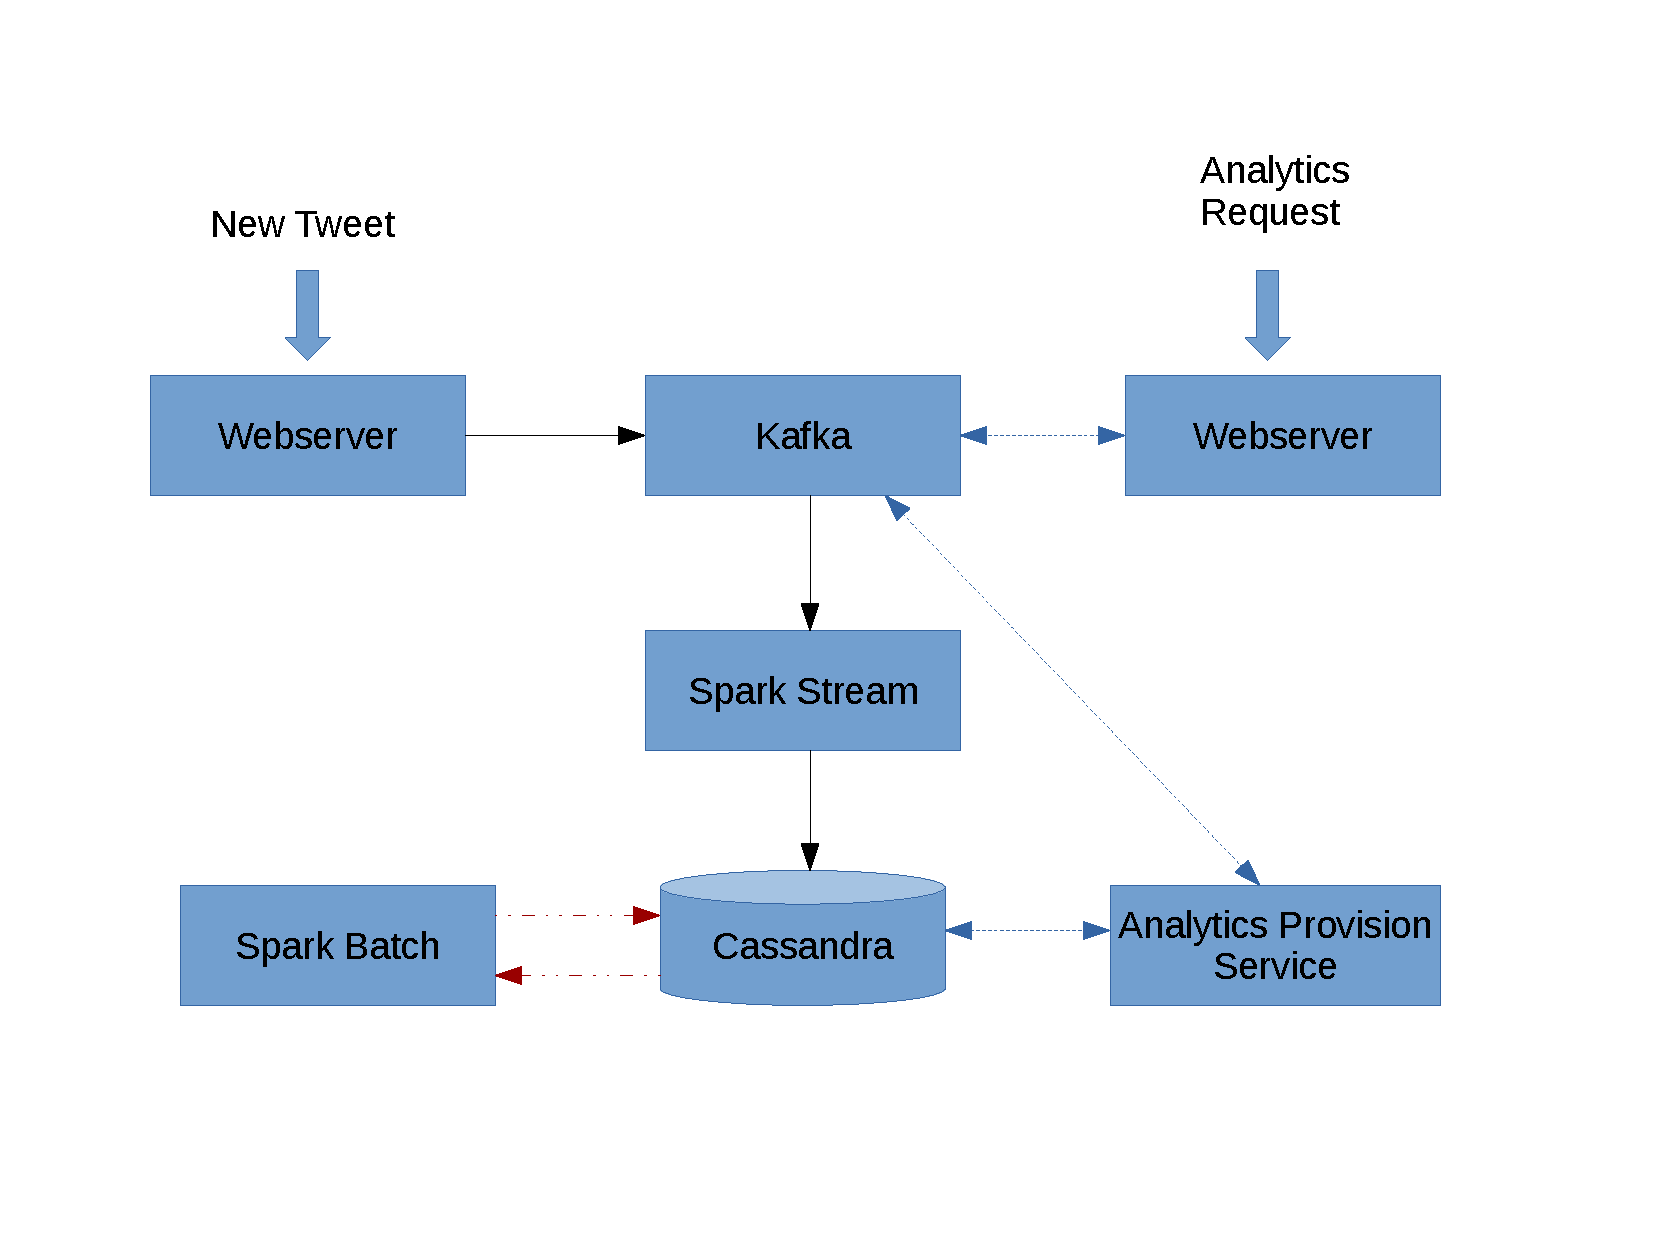
\includegraphics[width=\textwidth]{pics/analytics/archi}
	\caption{Übersicht der Analytics Komponenten}
\end{figure}

\section{Stream}

Die Streamverarbeitung innerhalb des Hamaube-Systems ist als eigenständiger Service geschrieben. Für die Umsetzung wurde SparkStreaming im Verbund mit Scala verwendet.

Folgende Ziele haben sich während des Projekt herausgebildet:
\begin{itemize}
	\item Vorverarbeitung der eingehenden Tweets für eine spätere Prozessierung mittels Spark
	\item Verarbeitung der Streamdaten für live Analyseergebnisse.
\end{itemize}


Als Input dienen bisher die beiden gegebenen Datenquellen:
\begin{enumerate}
	\item Tweets, welche aus der Twitter API in unsere Anwendung gestreamt werden.
	\item Hamaube-Tweets, welche in unserer Anwendung erzeugt werden.
\end{enumerate}

Auch die Streamverarbeitung ist über Kafka angebunden und erhält die Tweets über das \textit{USER\_ISSUES\_TWEET} Topic.


\subsection*{Vorverarbeitung für Spark Batch Processing}
Aus verschiedenen Gründen wurde für die Tweets im Hamaube-System das Datenmodell von Twitter übernommen.
Dadurch enthalten Tweets (vorallem solche, die direkt von Twitter kommen) eine Vielzahl von nicht gesetzten Feldern oder Daten, welche für die Analyse wenig interessant sind.
In der Vorverarbeitung wird nur ein definierter Teil der Felder eines Tweets übernommen und der Rest verworfen.
Zusätzlich werden (sofern vorhanden) die im Tweet enthaltenen Hashtags extrahiert und neben dem eigentlichen Tweet gespeichert.
Außerdem wird anhand des Tweet-Textes eine Sentiment Analyse durchgeführt, welche dem Tweet einen Score zuordnet, der dessen Stimmung widerspiegelt (negativ - negative Stimmung, positiv - positive Stimmung). Auch dieser Score wird neben dem eigentlichen Tweet gespeichert.

Wir haben uns dazu entschieden, die Tweetdaten zusätzlich - also dupliziert - zu den schon gespeicherten Tweets des 'CassandraReaders' in Cassandra zu speichern, da wir in Hinsicht auf ein produktives System die kritischen Tabellen nicht zusätzlich mit Anfragen belasten wollen.
Für die Analyse würde also ein separate Umgebung für Cassandra aufgebaut, dies haben im Hamaube-System aufgrund der Einfachheit noch nicht umgesetzt.

\subsection*{Live Analyse}
Zudem wird auf den durch Kafka eingehenden Tweetstream eine Live Analyse durchgeführt.
Das Spark Streaming Framework teilt den Stream dafür in Micro-Batches, die dann weiter verarbeitet werden können.
So werden z.B. die Anzahl von Hashtag pro Stunde/pro Minute ermittelt, daraus werden dann aktuell beliebte Hashtags erkannt.
Auch diese Ergebnisse werden in Cassandra gespeichert.
Um eine Skalierung zu ermöglichen müssen die Ergebnisse z.B. pro Stunde von mehreren Instanzen geupdated werden können, ohne dass dabei dirty reads oder Überschreibungen auftreten dürfen. Cassandra bietet hier den Datentyp \textbf{Counter}, der atomare \textit{increase} und \textit{decrease} Operationen anbietet. Damit lassen sich die meisten Szenarien realisieren, ohne weitere  komplexe (und möglicherweise verlangsamende) Isolierungsmechaniken zu implementieren.
\begin{figure}[htbp!]
\centering
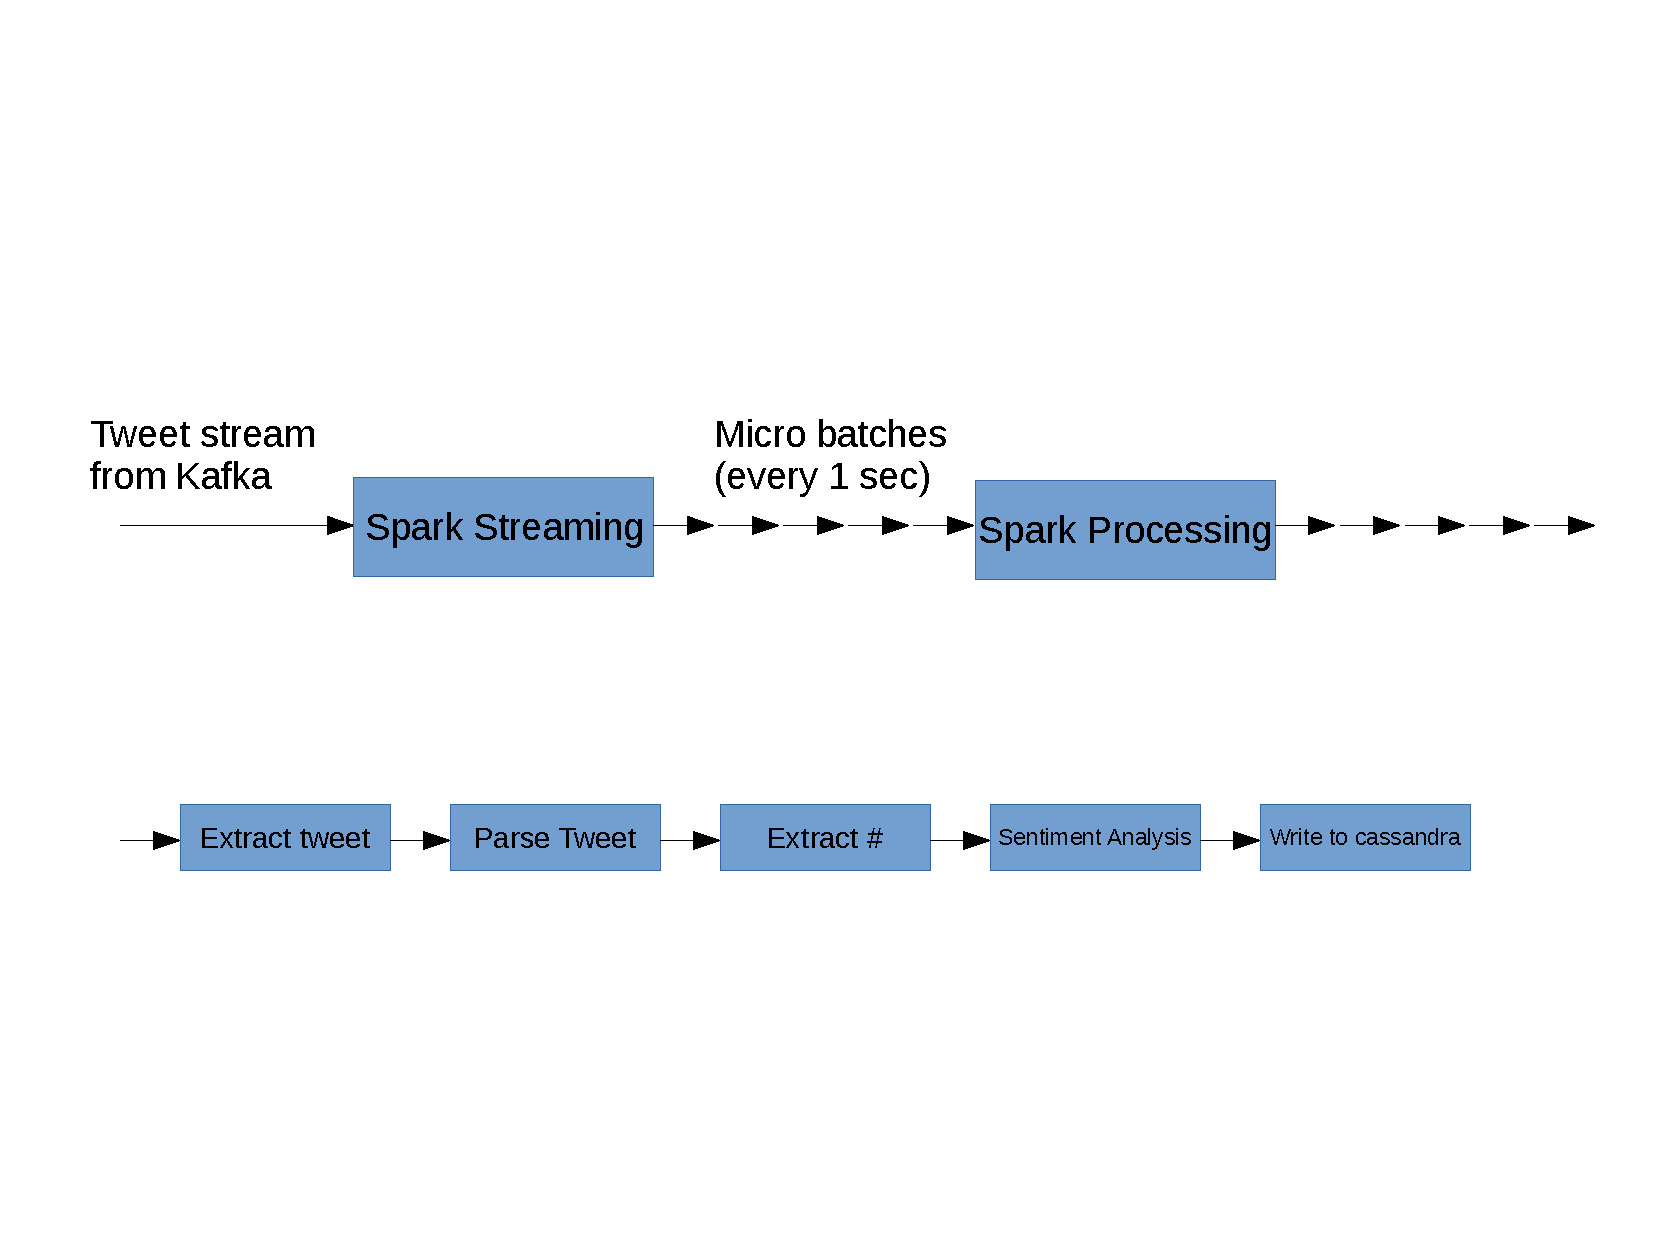
\includegraphics[width=\linewidth]{pics/analytics/streamProcessing.pdf}
\caption{Spark stream processing}
\label{fig:streamProcessing}
\end{figure}

\subsection*{Beispiel}

Der Spark Streaming Service erhält einen neuen Tweet aus dem Topic \textit{USER\_ISSUES\_TWEET}.
Dieser liegt im vom Twitter definierten Datenformat vor (Siehe \ref{chap:cassandra}).

Folgende Attribute werden für die Weitervearbeitung extrahiert:
\begin{itemize}
	\item Tweet-Id
	\item Tweet-Text
	\item User (Id, Name)
	\item Sensitivitäts-Flag 
	\item Hashtags
	\item Erstellungsdatum
	\item Sprache
	\item Ort (Land, Stadt)
	\item GPS-Koordinaten
\end{itemize}

Twitter extrahiert dabei die Hashtags aus dem Tweet-Text und schreibt diese zusätzlich in ein Entity-Objekt, welches am Tweet hängt.
Diese Hashtags können einfach genutzt werden und eine Extraktion aus dem Text wird vermieden.
Falls Werte nicht gesetzt sind oder ungültig sind, werden diese durch einheitliche Dummy-Werte ersetzt, welche in späteren Analysen erkannt und übersprungen werden.
Anschließend wird die Sentiment-Analyse des Tweet-Textes durchgeführt. Diese zählt anhand definierter Listen positive und negative Wörter im Text und berechnet daraus einen Score. Dieser Score kann später z.B. mit den zum Tweet gehörenden Hashtags analysiert werden, ein mögliches Szenario wäre ein Stimmungsbild zu einem bestimmten Hashtag.
Damit eingehende Tweets in Zeiteinheiten aggregiert werden können,
wird der Erstellungszeitpunkt eines Tweets auf entsprechende Zeiteinheiten abgerundet (z.B. Stunde, Minute). Für jede Zeiteinheit / Analyse-Target existiert in Cassandra eine Tabelle, für welche der Primary-Key als Verbund aus dem entsprechenden Analyse-Target (z.B. Hashtag) und der gerundeten Zeiteinheit vorliegt.
Dadurch lassen sich Updates effizient für jede Zeiteinheit / Analyse-Target durchführen.

\begin{figure}[htbp!]
	\centering
	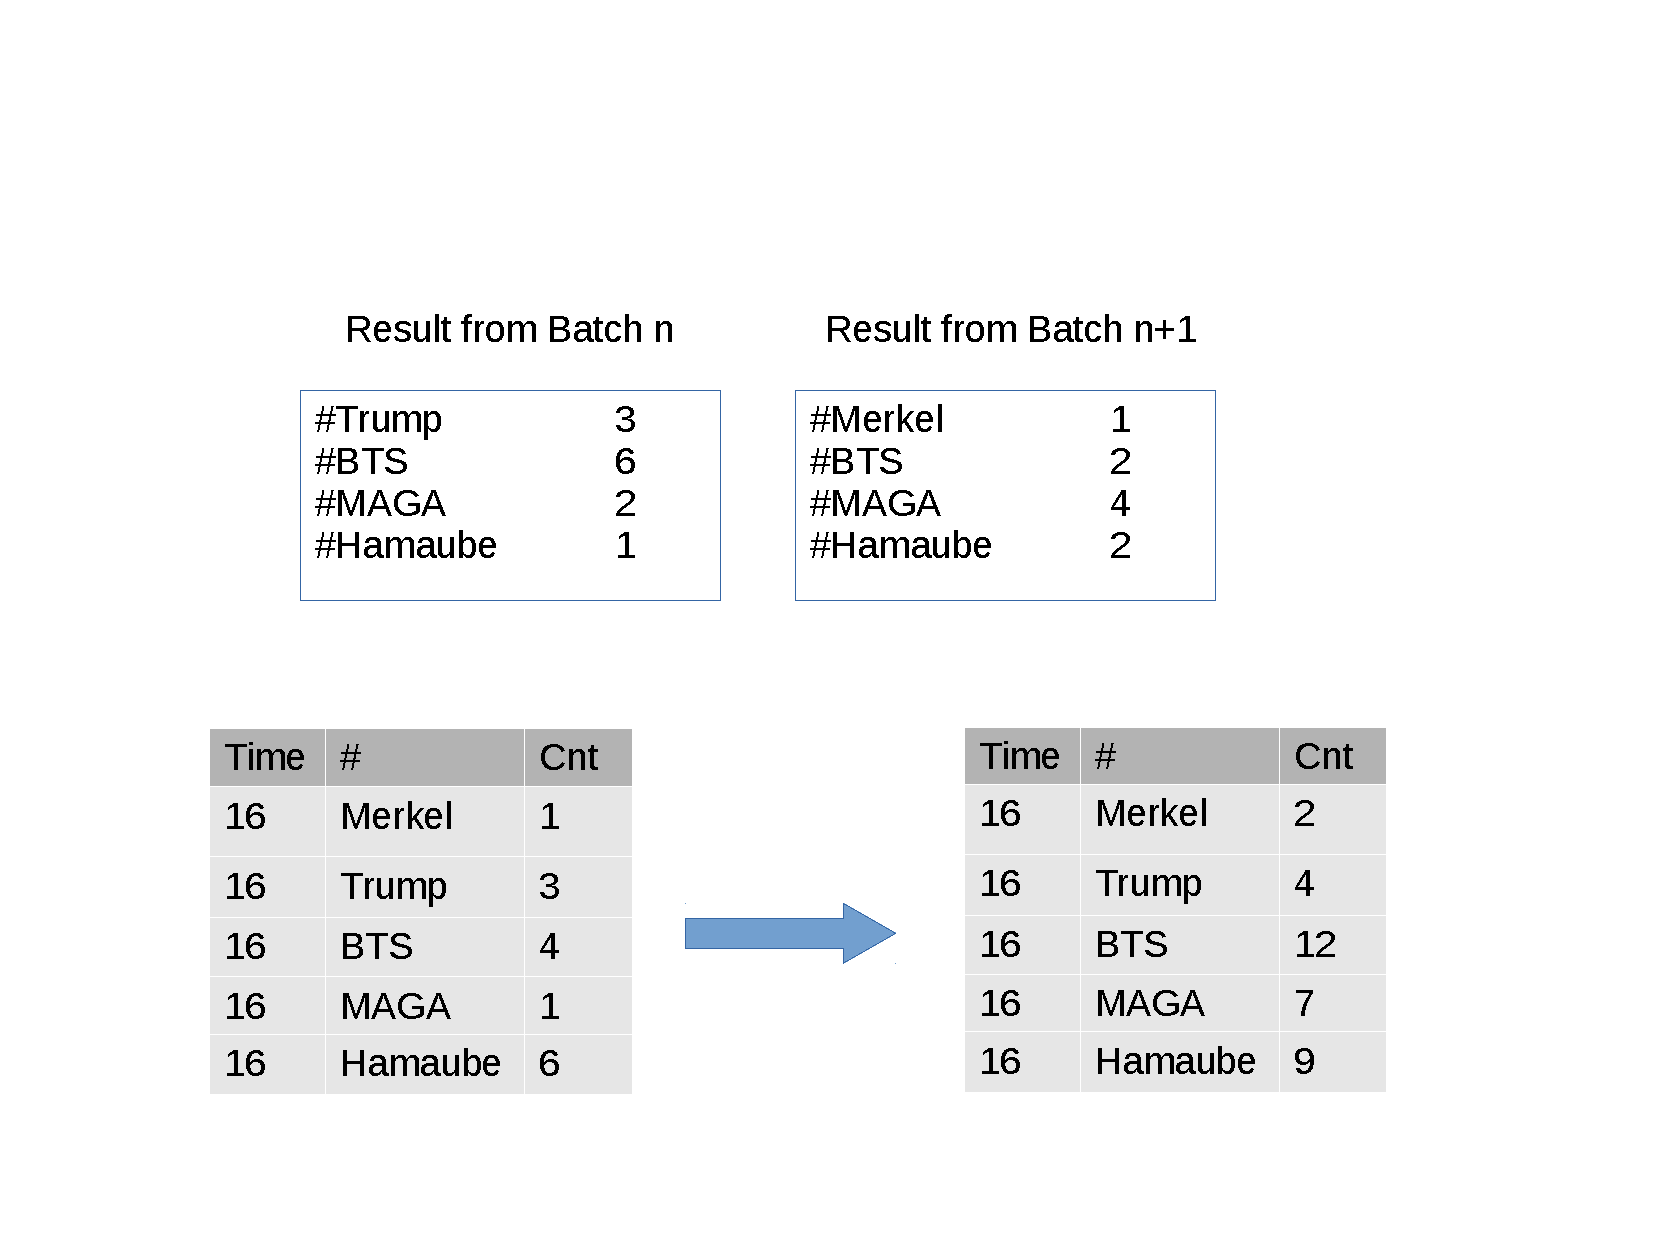
\includegraphics[width=1.1\textwidth]{pics/analytics/example}
	\caption{Sream Analytics: Beispiel - Anzal von Hashtags pro Stunde}
\end{figure}






% This file was converted to LaTeX by Writer2LaTeX ver. 1.0.2
% see http://writer2latex.sourceforge.net for more info
\documentclass{article}
\usepackage[utf8]{inputenc}
\usepackage[T1]{fontenc}
\usepackage[ngerman]{babel}
\usepackage{amsmath}
\usepackage{amssymb,amsfonts,textcomp}
\usepackage{array}
\usepackage{listings}
\usepackage{hhline}
\usepackage[pdftex]{graphicx}
\author{}
\date{2018-10-07T22:20:48.763142593}
\begin{document}
\section[Architektur]{\selectlanguage{ngerman} Architektur}
\subsection[zwei Phasen]{\selectlanguage{ngerman} zwei Phasen}
Die Ausführung der Analysen erfolgt in zwei Phasen. Die eine Phase ist
die eigentliche Batch-Analyse. Dabei werden alle bisher in der
Datenbank befindliche Tweets ausgewertet. Die andere Phase erfolgt
davor. Die Realtime-Analytics-Komponente überträgt die reinkommenden
Tweets in einer Art ETL-Prozess (extract, transform, load) in die
Datenbank. Dort werden sie in einem für die Analyse optimierten Format
gespeichert.

\subsubsection[ETL{}-Prozess]{\selectlanguage{ngerman} ETL-Prozess}
Der ETL-Prozess wurde ursprünglich notwendig, weil der
Cassandra-Connector für Spark einen Bug enthielt. Befanden sich an
speziellen Stellen im orginalen JSON-Objekt von Twitter NULL-Werte und
wurden diese in die Datenbank geschrieben, dann konnte der Connector
diese Objekte nicht korrekt verarbeiten. Die Tweets aus der Datenbank
werden auf ein Java-Objekt gemappt. Dabei wird versucht, alle Attribute
der Zielklasse mit Werten zu belegen. Dafür wird in der Datenbank nach
einer geeigneten, d.h. exakt gleich benannten Spalte gesucht. Dann wird
abhängig vom Datentyp der Spalte der gelesene Wert in den
entsprechenden Java-Typ umgewandelt. Der Bug tritt nun in der
Verschachtelung auf. Die JSON-Objekte können verschachtelt werden und
ebenso die Datenbank-Spalten. Dafür kann man zuerst den Datenbanktyp
selbst definieren und dann kann dieser als so genannter frozen-type
\ als normaler Spaltentyp genutzt werden. Wenn ein solches Objekt eines
frozen-types nun in der Datenbank als NULL abgespeichert ist, stolpert
der Connector darüber und findet keinen Umwandler von NULL zu einem
entsprechenden Java-Objekt.

Wir haben dann vom direkten Lesen der Tweets aus dem Datenbankteil, in
dem der Webserver sie schreibt, auf Lesen der Tweets aus einem eigenen
Datenbankteil umgestellt. Die Tweets kommen über Kafka an den
Realtime-Analytics-Prozess, der diese auswertet (extract). Der
zugehörige Kafka-Connector enthält keinen solchen Bug.

Vor dem Laden in die Datenbank wird der Tweet nun stark reduziert, d.h.
es werden viele Felder entfernt, die für die Analyse gar nicht benötigt
werden. Zudem werden die NULL-Werte an den kritischen Stellen durch
Dummy-Objekte ersetzt (transform). Schlussendlich werden sie vom selben
Cassandra-Connector in die Datenbank geschrieben, mit dem sie später
auch gelesen werden. (load).

Neben der nun vorhandenen Kompatibilität mit dem Cassandra-Connector
führt der ETL-Prozess auch zu deutlich kleineren Tweet-Objekten, was
die Analyse stark beschleunigt, insbesondere wenn die Tweets über das
Netzwerk übergeben werden müssen.

\subsubsection[eigentliche Analyse]{\selectlanguage{ngerman} eigentliche
Analyse}
Nach dem ETL-Prozess kommt die eigentliche Analyse. Der ETL-Prozess wird
ständig von der Streaming-Komponente ausgeführt, d.h. es werden Tweets
sekündlich in die Datenbank geladen.

Die eigentliche Analyse, eine Batch-Analyse wird regelmäßig, z.B. nachts
durchgeführt. Sie dauert auch deutlich länger, sie könnte gar nicht in
Echtzeit erfolgen. Ziel der eigentlichen Analyse ist es, statistische
Werte über die Aktivität der User und Inhalte der Tweets zu ermitteln.
Hierbei geht es um die Gesamtheit der Tweets. Desweiteren werden
weitere Parameter ermittelt und Empfehlungen vorbereitet. Diese
beziehen sich auf einzelne Tweets bzw. User.

\section[Skalierbarkeit]{\selectlanguage{ngerman} Skalierbarkeit}
Übergeordnetes Ziel dieses Projektes ist ja die Implementierung in einer
skalierbaren und erweiterbaren Architektur. Das Prinzip dafür lautet:
nutze skalierbare Komponenten und verbinde sie skalierbar. Mit
skalierbar ist hier scale-out gemeint, d.h. die Daten aus der Datenbank
liegen auf verschiedenen Servern vor. Die Datenbank kümmert sich um die
Verteilung der ihr zugeführten Daten. Cassandra skaliert durch die
Verteilung der Daten auf verschiedene Server. Ähnlich skaliert Spark.
Spark wird ebenso auf verschiedenen Rechner ausgeführt, die zusammen
als Cluster die Analyse ausführen. Dabei werden die Daten auf dem
Rechner gehalten, der auch die Analyse durchführt. So weit, so gut.
Allerdings gibt es hier nun einen Stolperstein, der die Skalierbarkeit
gefährdet. Die Daten liegen bisher in Cassandra und müssen zu den
Spark-Rechnern übertragen werden. Hier gibt es nun drei denkbare Wege:

\begin{itemize}
\item die Daten werden von einem Koordinator aus Cassandra abgerufen und
in Sparks verteiltes Dateisystem geladen. Offensichtlich ist dieser
Koordinator ein Flaschenhals. Dieser Fall sollte dementsprechend
vermieden werden, erfordert aber einen eigenen Sparkconnector zu
Cassandra.
\item die Daten werden von den einzelnen Spark-Rechner passend
abgerufen, d.h. jeder Spark-Rechner ruft die für ihn notwendigen Daten
ab und die Analyse wird so verteilt, dass diese Datenmengen
untereinander überschneidungsfrei sind.
\item die Berechnung folgt den Daten. Die Analyse von Spark wird auf den
Rechner ausgeführt, auf denen auch Cassandra die Daten hält. Dann
würden sie nur auf dem Rechner übertragen. Offensichtlich würde diese
Variante besonders wenig Netzwerktraffic generieren. Allerdings würde
die Rechnenlast auf den Cassandra-Knoten steigern. Wenn diese Knoten
nun auch die Produktiv-Knoten für die Datenbank des Frontends wären,
müsste man diese Effekte abwägen. Hat man allerdings eine eigene
Datenbank bzw. einen eigenen Keyspace für die Analysen, so müsste man
diese Effekte nicht gegeneinander abwägen. Und wir haben ja einen
solchen Keyspace für die Analysen, der mit dem ETL-Prozess gefüllt wird.
\end{itemize}
Wir verwenden einen Cassandra-Connector in Spark, der das letzte Prinzip
versucht. Er versucht die Analysen möglichst auf dem gleichen Knoten
auszuführen, auf dem auch die Daten in Cassandra liegen. Möglich wird
dies dadurch, dass man diese Informationen aus Cassandra abrufen kann
und dass Spark die Möglichkeit bietet, die Verteilung der Analysen
genau aus solchen Gründen zu beeinflussen. In unserem Testsetup
funktioniert das leider nicht, da keine gesonderten Knoten für die
Analytics-Cassandra-Instanz zur Verfügung stehen und Spark auf anderen
Knoten läuft. Damit entspricht unsere skalierbare Verbindung der aus
dem zweiten Fall.

Der dritte Fall, auch genannt Datenlokalität, ist nicht unbedingt der
bessere. Nicht nur, wenn die Datenbankknoten noch mit anderen Dingen
beschäftigt sind, nein auch, wenn die Analyse im Vergleich zum Laden
der Daten komplexer wird, also mehr Rechenleistung benötigt wird.
Ausprobiert wurde deshalb auch, wie sich unsere Analysen verhalten,
wenn man sie zwar auf mehr CPU-Kernen ausführt, dafür aber ein
langsameres Netzwerk simuliert. Die Anzahl parallel laufender Einheiten
ist deutlich sichtbar. Es werden so viele Einheiten gleichzeitig
fertig, wie der Prozessor Kerne hat. In diesem Fall zeigt aber eine
Auswertung der CPU-Last, dass die Übertragung über das Netzwerk der
Flaschenhals ist, denn die CPU-Kerne sind max. zu Hälfte ausgelastet.
Ist das Netzwerk schneller, dann steigt auch die CPU-Auslastung auf
nahezu 100\%.

\subsubsection[mit Flaschenhals]{\selectlanguage{ngerman} mit
Flaschenhals}

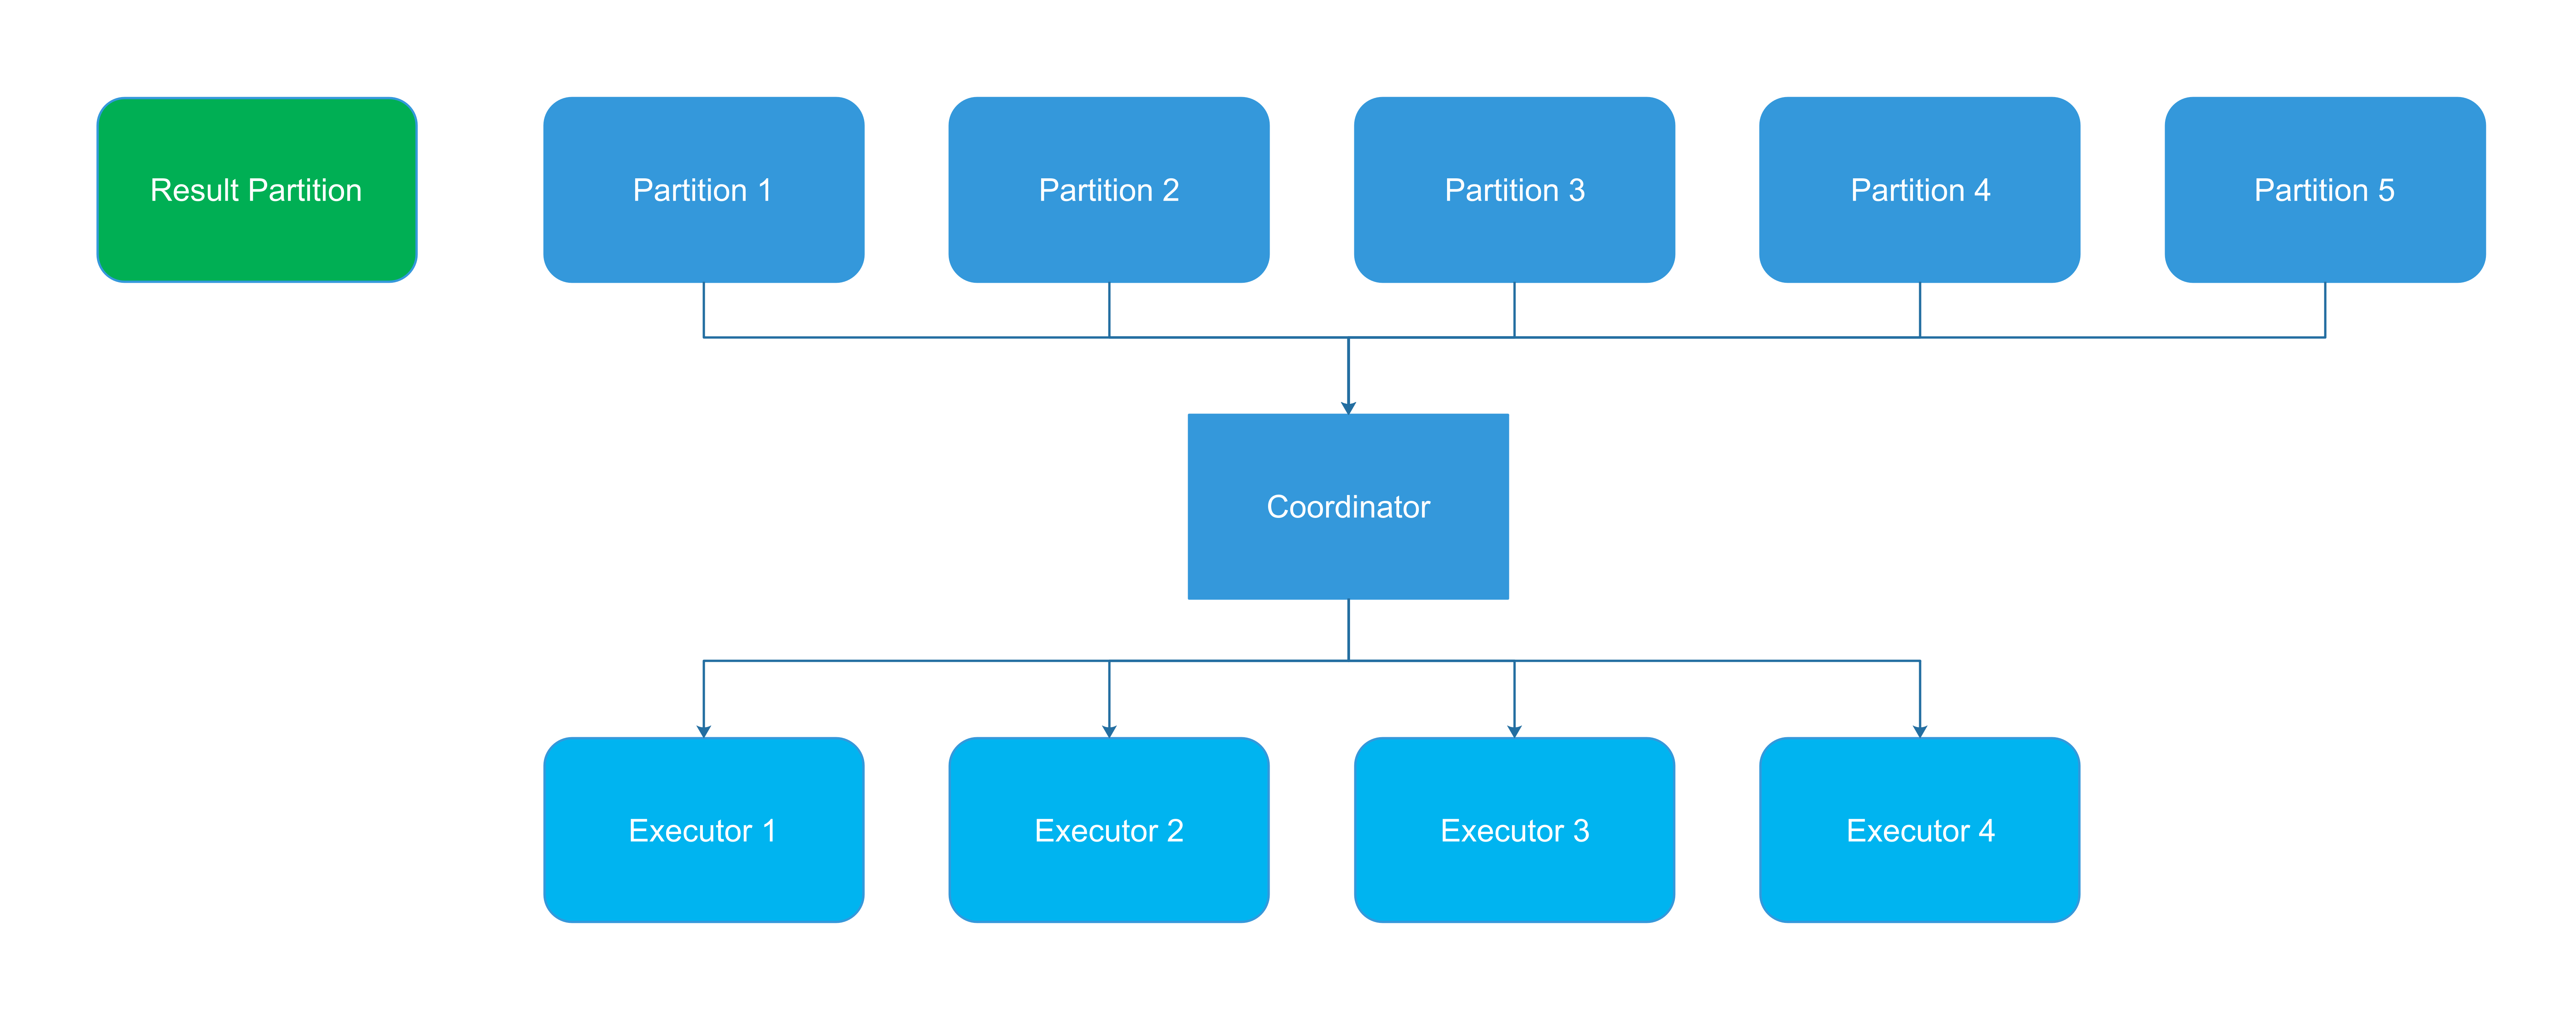
\includegraphics[width=15.24cm,height=5.99cm]{bilder/eigene20PrC3A4sentation-img1.png}


\subsubsection[Durcheinander]{\selectlanguage{ngerman} Durcheinander}

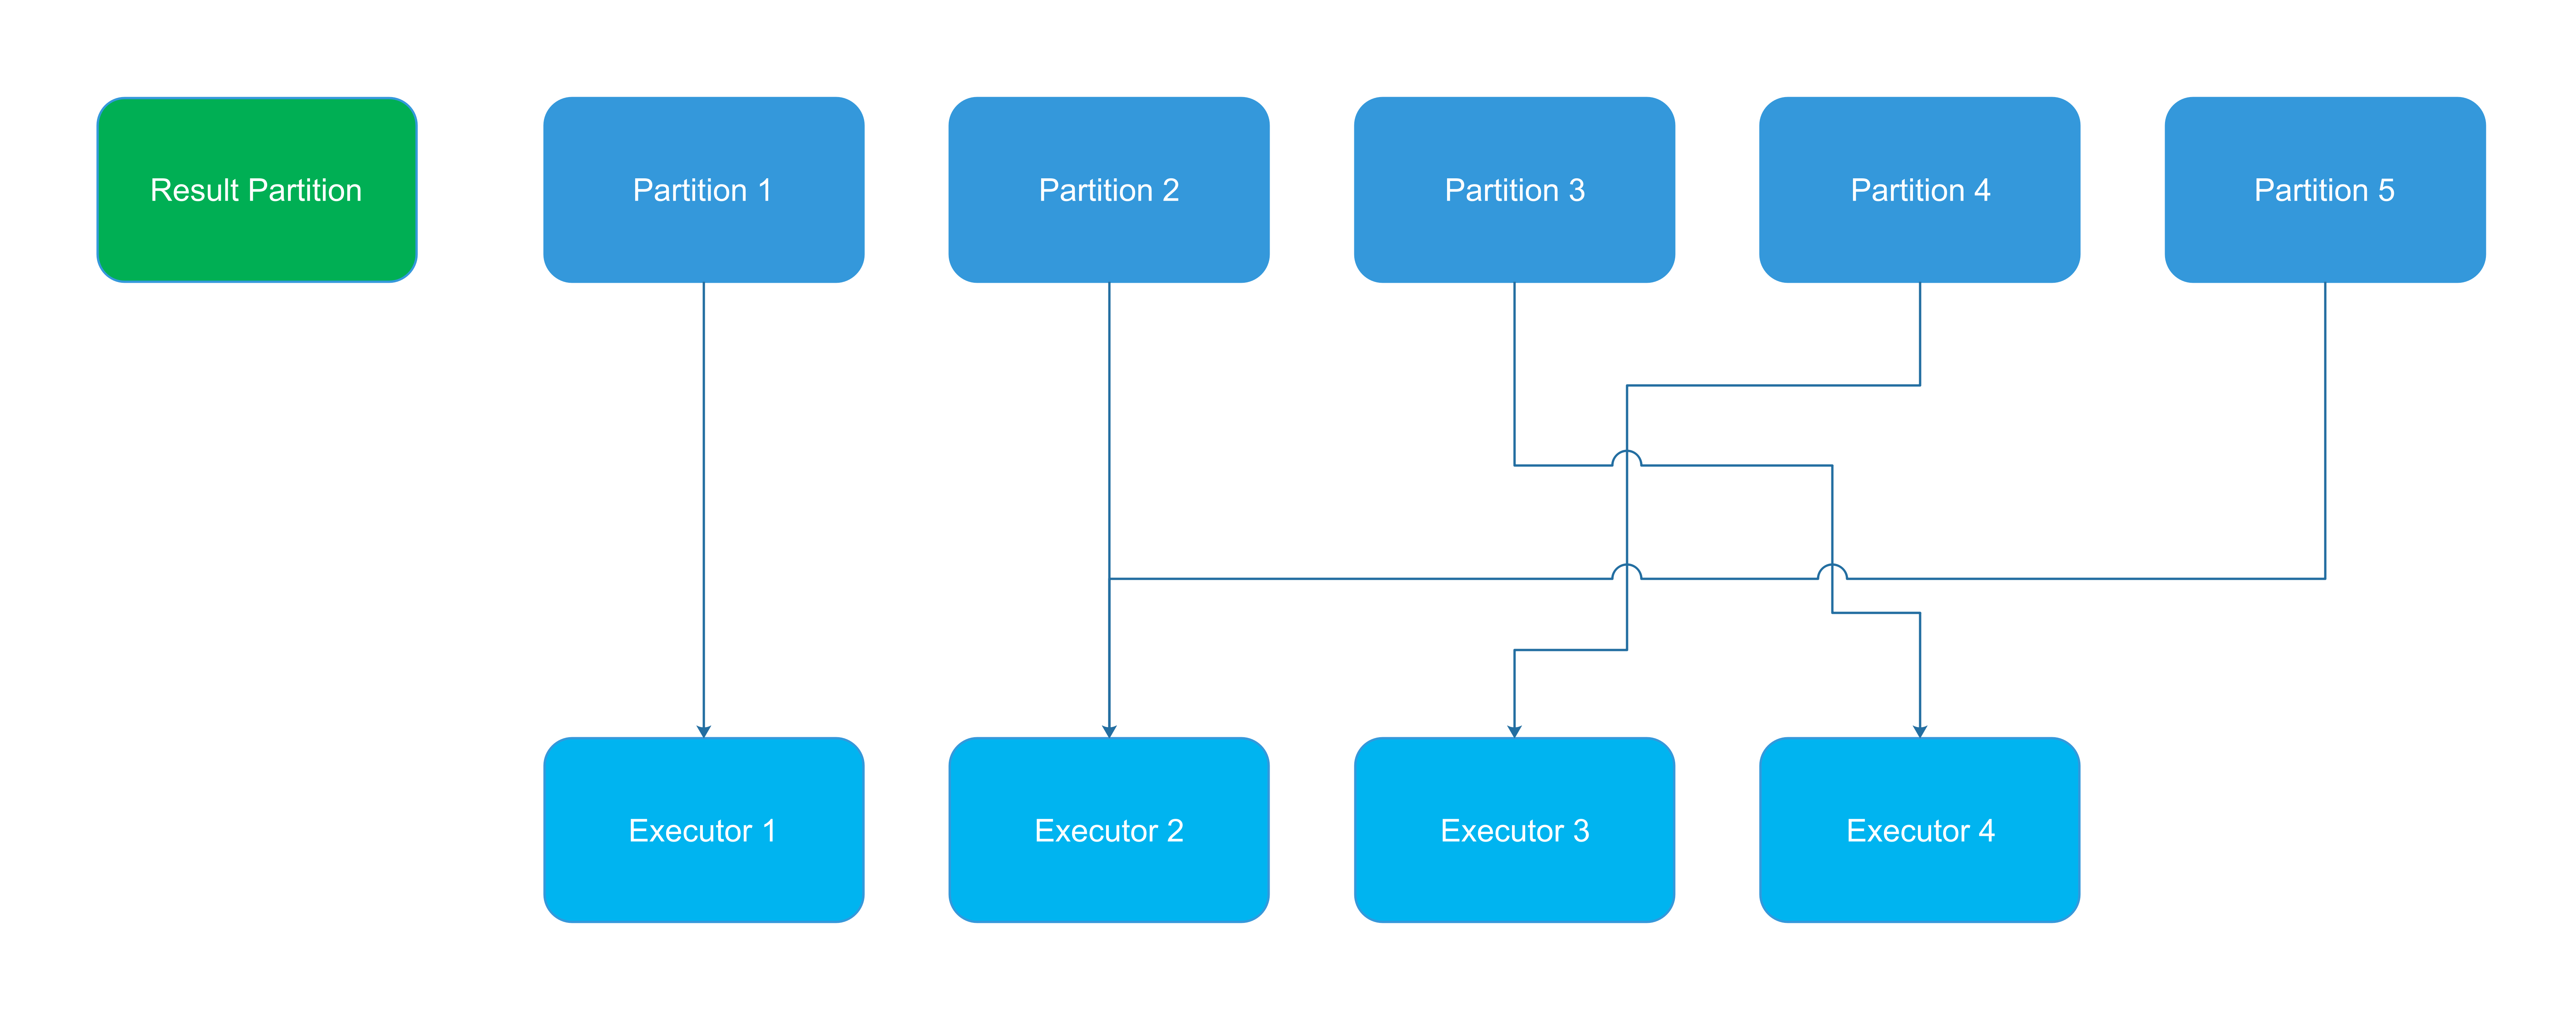
\includegraphics[width=15.24cm,height=5.99cm]{bilder/eigene20PrC3A4sentation-img2.png}


\subsubsection[mit Data Locality]{\selectlanguage{ngerman} mit Data
Locality}

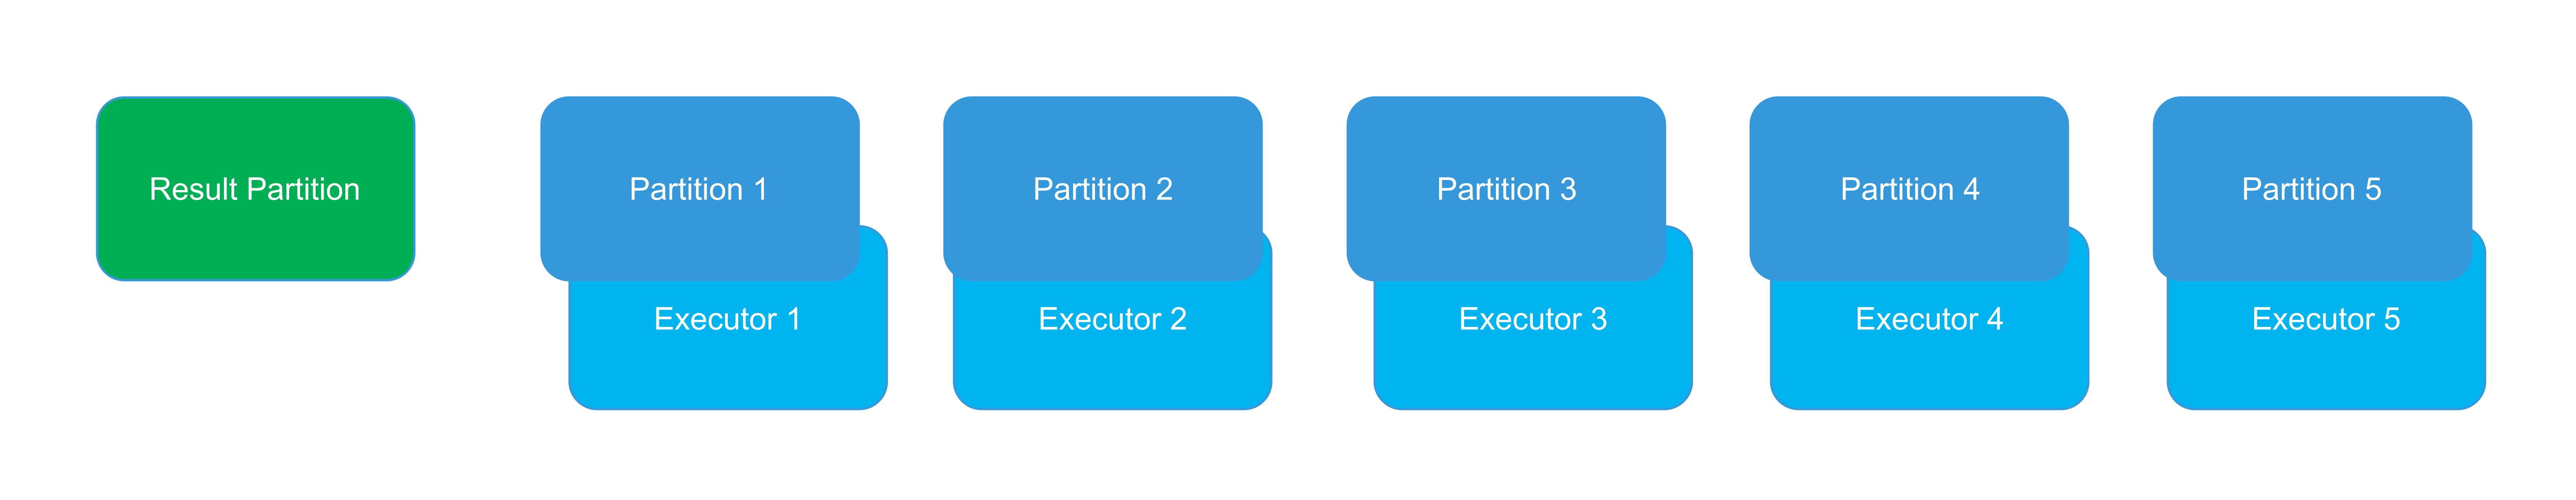
\includegraphics[width=15.24cm,height=2.956cm]{bilder/eigene20PrC3A4sentation-img3.png}


\section[Use{}-Cases]{\selectlanguage{ngerman} Use-Cases}
Die Batch-Analytics-Komponente hat vorrangig das Ziel, inhaltlich
relevante Entwicklungen in den Tweets zu zeigen. Das wären z.B. länger
trendende Hashtags zu identifizieren.

Folgende statistische Werte werden erhoben und im Frontend angezeigt:

\begin{itemize}
\item Gesamtanzahl Tweets
\item Anzahl fröhlicher Tweets (gemessen am Vorliegen eines Smileys) und
Anzahl trauriger Tweets (Vorliegen eines Sadleys)
\item \ die Anzahl Tweets pro Tag
\item \ die Top 10 Hashtags pro Tag
\item \ die Top 10 Stunden mit dem meisten Tweets pro Tag
\item \ die Top10 Tweeter pro Tag
\item sowie die Top 10 verwendeten Wörter pro Tag.
\end{itemize}
Eine Vorstellung der Ergebnisse findet sich weiter unten.

Diese Daten werden von Spark ermittelt und in eine Ergebnistabelle von
Cassandra geschrieben. Dort werden sie vom AnalyticsServices bei
Anfrage durch den Webserver ausgelesen und an den Webserver gesendet.
Dieser wiederum leitet sie an das Frontend weiter, wo sie mittels
Javascript grafisch dargestellt werden.

Weiterhin sind folgende Anwendungen in Spark implementiert:

\begin{itemize}
\item Analyse der Tweetsprache durch Analyse der vorkommenden
Stopwords
\item Ermittlung von zeitlichen Aktivitätsprofilen der User
\item Ermittlung von Association-Rules für das Folgen von Nutzern.
\end{itemize}
Die erste beiden Komponenten werden im Frontend nicht aktiv eingesetzt.
Die letzte Komponente kann nicht sinnvoll benutzt werden, da im
Gegensatz zu den vielen Tweets unsere Userdaten sehr lückenhaft sind.
Es fehlen die Informationen über die gefolgten Nutzern bzw. nur ein
Nutzer in unserer Datenbank hatte mehr als einen Follower. Damit ließen
sich keine Association-Rules generieren. Der einzige Nutzer, dem mehr
als ein Nutzer folgt (zwei Nutzer) ist der Twitter-Account der
übermäßig präsenten koreanischen Boyband BTS. Sie wird später nochmal
genauer angeschaut.

Ein weiterer Usecase für die grafischen Analysen ist die Überprüfung der
Funktionsweise des Systems. Werden die Daten aufgrund einer
Schema-Änderung bei Twitter nicht mehr in die Datenbank gespeichert, so
würde man dies in den Analysen sehen können. Auch ein
Programmierfehler, bei dem der Benutzername nicht richtig übertragen
wurde, fiel auf. Statt Tweetern mit ca. 40-80 Tweets pro Tag tauchte in
den Top 10 der Tweeter nur ein Nutzer auf, nämlich NULL.

Ein dritter Usecase fällt bei der Analyse der Top-Hashtags auf. Am
27.09. z.B. ist einer der Top10-Hashtag PCA. Das steht für
People{\textquotesingle}s Choice Award. Es handelt sich hierbei um eine
Online-Abstimmung, die durch Nennungen in den sozialen Medien erfolgt.
Zur Auswertung ist eine solche Gesamtanalyse natürlich nötig.

\subsection[Erkenntnisse durch grafisch aufbereite
Statistiken]{\selectlanguage{ngerman} Erkenntnisse durch grafisch
aufbereite Statistiken}
Wir haben eine einfache Sentiments-Analyse eingebaut. Ziel ist es, die
insgesamte Stimmung auf einer Skala von positiv bis negativ einordnen
zu können. Die Sentiments-Analyse wertet die Tweets auf das Vorkommen
von Smileys :-) und Sadleys :-( aus. Die jeweilige Gesamtzahl wird dann
angezeigt. Diese Methode ist offensichtlich ziemlich ungenau und das
zeigt sich auch in den Ergebnissen. Am 1.10.2018 hatten wir fast 10
Millionen Tweets in der Datenbank, aber nur 2177 enthielten ein Smiley
und sogar nur 366 ein Sadley.

Hier zeigt sich auch beispielhaft, warum eine Arbeitsteilung zwischen
Datenbank und Analysen sinnvoll sein kann. Die Datenbank kann nämlich
nicht ausgeben, wie viele Tweets in ihr speichert sind. Die
entsprechende Anfrage timed out. Für andere Anfragen ist ein geeigneter
Index notwendig. Dessen Notwendigkeit ist nicht immer im Voraus bekannt
und eine Nachrüstung kaum möglich.

\section{\selectlanguage{ngerman}
interessante Analyseergebnisse}
\subsection[BTS]{\selectlanguage{ngerman} BTS}
Bei unseren Analysen war der Hashtag BTS in verschiedenen Formen immer
präsent. BTS steht für Bangtan Boys und ist eine koreanische Boyband.
Ihre hohe Präsenz auf Twitter ist nicht nur Folge hoher Popularität und
der Auswahl durch Twitter, sondern auch Ergebnis diverser
Social-Media-Kampangen. BTS startete unter anderem die
LoveYourself-Kampange. Ziel derer ist es, die Liebe in der Welt zu
verbreiten. Aussage ist es, dass für die Liebe in der Welt zuerst die
Selbstliebe notwendig ist. Diese Jahr sprachen sie vor den Vereinten
Nationen zu diesem Thema. Ein weiterer Hashtag aus dem BTS Umfeld ist
deren A.R.M.Y, was für Adorable Representative M.C for Youth steht.
Damit wird ihr Fanclub bezeichnet.

Eine These, warum es gerade BTS so konstant in unsere Tweets schafft,
ist dass unser Selektionskriterium love diese LoveYourself-Kampange
trifft.


\includegraphics[width=15.24cm,height=8.557cm]{bilder/eigene20PrC3A4sentation-img4.png}

\bigskip

\subsection[Twitter{}-Spam]{\selectlanguage{ngerman} Twitter-Spam}
Die Analyse der Top 10 Tweeter am 23. und 24.09.2018 zeigt ein weiteres
interessantes Phänomen: den Twitter-Spam. Mit der Möglichkeit sich an
bekannte Hashtags hängen zu können, zieht Twitter auch Spammer an. Am
24.09.(und am 23.09) \ hat es eine Gruppe von Usern geschafft, durch
jeweils 30 Tweets pro Nutzer unsere Top 10 mit Porno-Spam zu füllen,
mit User wie DAILY HOMEMADE, und THE PORN PROMO LIST. In den
darauffolgenden Tagen tauchen sie dann nicht mehr auf, was für
Gegenmaßennahmen auf Seiten Twitters spricht. Am 01.10.2018 tauchen sie
dann langsam wieder in den Top 10 auf.

\subsection[Trump related]{\selectlanguage{ngerman} Trump related}
In unseren Daten sind jeden Tag große Mengen von Tweets über/mit Donald
Trump enthalten. Neben seiner bekanntermaßen hohen Twitterpräsenz liegt
das auch an dem Selektionskriterium, mit dem wir bei Twitter nach
Tweets anfragen. Es enthält unter anderem den Selektor Trump.

\section[spezielle Analyseergebnisse]{\selectlanguage{ngerman} spezielle
Analyseergebnisse}
\subsection[stream{}-bedingte Ergebnisse]{\selectlanguage{ngerman}
stream-bedingte Ergebnisse}
Es gibt einige Gründe, die unsere Analyseergebnisse verzerren.

Der erste Grund ist die konstante Geschwindigkeit unseres
Twitterstreams. Offensichtlich verarbeiten wir nicht 100\% der Tweets
weltweit oder auch nur deutschlandweit. Stattdessen lassen wir uns von
Twitter über deren API eine Auswahl geben. Die API liefert maximal 80
Tweets pro Sekunde aus. Wir haben diese Rate auf 2 Tweets pro Sekunde
limitiert. Am 24.09.2018 kommen alle
Stunden auf $7918 \pm 5$ Tweets. Das entspricht gerade
der Streamgeschwindigkeit.

Zudem lassen z.B. am 01.10 auch die Auswirkung der Analysezeit sehen. An
diesem Tag lief der Stream nur zeitweise und genau diese Zeiten lassen
sich erkennen. Er wurde irgendwo zwischen 10 und 11 Uhr angeschaltet
und lief zwischen 11 und 12 wieder vollständig (ca 7200 Tweets). Nach
12 Uhr wurde er wieder unterbrochen und ca.zwischen 14:30 und 15:40
lief er dann wieder. 

\subsubsection[Sampling verzerrt die absoluten
Zahlen]{\selectlanguage{ngerman} Sampling verzerrt die absoluten
Zahlen}
Bei manchen Analysen, z.B. Tweets pro Tag stimmen die absoluten Zahlen
nicht. Am 24.09.2018 weist die Grafik 353 Tweets aus. Wir wissen aber
durch die Auswertung über die Stunden das es ca. 172800 Tweets sein
müssten (24 Stunden x 7200 Tweets pro Stunde). Das liegt daran, das
für die Grafik ein Sampling der Tweets genommen wurde, d.h es wurde nur
ein Bruchteil analysiert. Während der Entwicklung dient das dazu, dass
die Analysen schnell ausgeführt werden können (ca. 1 Minute vs. 20
Minuten). Im Produktivbetrieb würde man dieses Sampling dann nicht mehr
vornehmen.

\section[genauere Schritte]{\selectlanguage{ngerman} genauere Schritte}
Ein großes Hindernis bei der Entwicklung und dem Betrieb der Analysen
war es, dass die Beispiele und gefundenen Howtos zu einfach sind. Im
Sinne einer gewissen Wissensweitergabe sollen hier anhand einiger
Patterns – analog zu Design Patterns – die gewonnen Erkenntnisse
weitergegeben werden. 

\subsection[doppelter Key]{\selectlanguage{ngerman} doppelter Key}
Eine Herausforderung war es, dass der Mapping-Schritt zwar ein
Key-Value-Mapping vornimmt, aber nur einen Key unterstützt. Für die
Analysen wird aber häufig ein mindestens doppelter Key benötigt. Zum
Beispiel wenn die Top 10 Tweeter pro Tag bestimmt werden sollen. Dann
sieht ein typisches Key-Value-Paar eigentlich so aus (Tag, Tweeter →
1). Die beiden Angaben für den Key lassen sich einfach aus den Tweets
extrahieren. Nun müssen sie noch verbunden werden. Die einfachste
Möglichkeit, die funktioniert hat, ist die beiden Angaben jeweils in
einen String zu exportieren und die beiden Strings zu konkatenieren.
Damit die beiden Teile später wieder getrennt werden können, muss noch
ein eindeutiges Trennzeigen eingefügt werden. Kein einzelnes Zeichen
kann dafür verwendet werden, da sie alle potentiell in den Tweets
vorkommen können. Wir verwenden deshalb eine lange, zufällige
Zeichenkette, wie sie so wohl kaum in einem Tweet vorkommen wird.

Eine weitere Methode wäre es, eine eigene Klasse für das Key-Value-Paar
zu erstellen. Hierbei ist darauf zu achten, sowohl equals() als auch
hashCode() korrekt zu implementieren.

Eine dritte Möglichkeit wäre es, das in Scale eingebaute Tuple2 zu
verwenden.

Keine Möglichkeit war es, bereits zu Anfang die Daten aufzuteilen und
zuerst nach Tagen zu filtern und dann 14 Analysen laufen zu lassen. Das
würde zu lange dauern, da Spark die Daten dann zu häufig anfordern
würde (nämlich neu für jeden Tag).

Auch deshalb wäre eine bessere Unterstützung durch Spark hier sinnvoll.
Denn es gibt einen weiteren Fall, der ganz ähnlich ist.

\subsection[Top10 pro Tag nehmen]{\selectlanguage{ngerman} Top10 pro Tag
nehmen}
Unsere Analysen sind häufig pro Tag. Das bedeutet, dass wir die Top 10
für die letzten 14 Tage zum Beispiel nehmen wollen. Wir brauchen also
14 Top 10s. Die eingebaute Sortierung kann einem hier nur teilweise
helfen. Sortiert man wie normal nach Values, so ist nicht garantiert,
dass sich die Top 10 der 14 Tagen überhaupt am Anfang findet. Werden an
einem Tag besonders viele Tweets abgesendet, so verdeckt das natürlich
die anderen Tage. Die sortierte Liste enthält dann viele Einträge
der aktiveren Tage und die Top 10 der weniger aktiven Tage findet sich
weiter hinten.

Die einzige korrekte Lösung, die wir gefunden haben, ist es sich die
gesammte Liste nach dem Reduce auf einem Knoten zusammenführen zu
lassen und sie dann von oben nach unten zu iterieren. Bei der Iteration
übertragen wir das gesichtete Element die Top10 des entsprechenden
Tages, so lange der Tag nicht schon 10 Einträge in der Liste hat.

Dieses Verfahren ist allerdings unnötig wenig parallelisiert. Würde man
die Daten früh nach Tagen shuffeln, so könnte man diese Operationen
zumindest nach Tagen parallelisiert auf unterschiedlichen Knoten
ablaufen lassen.

Wahrscheinlich gibt es dafür eine Lösung in Spark. Eine einfache
Unterstützung für die Unterteilung von Daten in einzelne Klassen und
dann Durchführung der selben Operation für alle Klassen separat wäre
trotzdem sehr hilfreich. \ 

\subsection{\selectlanguage{ngerman} Bausteine}
Man sagt, dass Spark mit dem Map-Reduce-Paradigmum verwendet wird. Die
Daten werden eingelesen und auf ein Ergebnis oder einen Fall gemappt
und diese dann aggregiert (reduce). Während der Arbeit an den
Batch-Analytics wurde deutlich, dass etwas mehr Schritte vorgenommen
werden müssen. Konkret fielen die Schritte:

\begin{itemize}
\item Daten laden
\end{itemize}
Die Grundoperation für das Laden der Daten ist beim verwendeten
Cassandra-Connector der Table-Scan. Komplexere Abfragen lassen sich
(noch) nicht ausführen. Damit kann keine Selektion nach einem Kriterium
erfolgen (zum Beispiel Tweets der letzten vierzehn Tage). Diese
Selektion muss dann im Filter-Schritt erfolgen.

\begin{itemize}
\item ggf. samplen
\end{itemize}
Gerade während der Entwicklungszeit ist es ratsam, darüber nachzudenken
zuerst die Analysen mit einem (sehr) kleinen Ausschnitt der Daten
durchzuführen. Dafür kann das entstandene RDD entweder gesampelt werden
oder n Elemente davon genommen werden (take). Das erste Fall ist durch den
Salt für den Pseudo-Zufallsgenerator deterministisch, das zweite nicht.
Das erste dauert ähnlich lange wie das Laden der ganzen Daten,
insbesondere ist es unabhängig von dem Anteil der zu holenden Daten. Das
zweite, das Taken, erfolgt viel schneller. Hier werden keine weiteren
Daten mehr übertragen, sobald die gewünschte Anzahl erreicht ist. Die
Daten könnten aber weniger stark durchmischt sein.

Da unsere Operationen nicht besonders teuer sind, hat das Samplen kaum
einen Geschwindigkeitsvorteil gebracht. Für das reine Testen der
Funktionalität konnte das Taken aber mit hohem Geschwindigkeitsvorteil
eingesetzt werden.

\begin{itemize}
\item \ Filtern
\end{itemize}
Dieser Schritt ist deshalb nötig, weil die Grundoperation der Table-Scan
ist. Es können aber auch unnötige Tweets aussortiert werden, z.B.
Tweets, die nicht zu einem gewissen Thema gehören.

\begin{itemize}
\item Mappen
\end{itemize}
Der bekannte Map-Schritt. Häufig werden mehrere Eigenschaften der
Gesamtheit untersucht. Das lässt sich dadurch bewerkstelligen, dass man
ein Vektorobjekt mit Feldern für alle untersuchten Eigenschaften anlegt
und für diese separat die Werte berechnet.

\begin{itemize}
\item Reducen
\end{itemize}
Der bekannte Reduce-Schritt. Hat man während des Mappen-Schritts ein
Vektorobjekt angelegt, so muss man hier auch wieder eine Vektorreduktion
vornehmen.

\begin{itemize}
\item Ergebnis produzieren
\end{itemize}
Nach dem Reduce liegen noch ggf. viele Daten vor. Bei der Analyse der
Top Hashtags liegen z.B. zu allen überhaupt vorkommenden Hashtags die
Häufigkeiten vor. Diese müssen jetzt noch weiterverarbeitet werden, indem
 z.B. die gewünschten Daten extrahiert werden (Top 10 der letzten
vierzehn Tage).

\begin{itemize}
\item und Ergebnis abspeichern
\end{itemize}
Die Daten müssen noch zum Zwecke der Persistenz in Cassandra geschrieben
werden.

auf.


\bigskip

\section[Verbesserungsvorschläge]{\selectlanguage{ngerman}
Verbesserungsvorschläge}
Bei der Arbeit an der Spark-Komponente sind einige
Verbesserungsvorschläge aufgekommen. Man sieht deutlich, dass es sich
bei Spark und Cassandra noch nicht um jahrzehntelang erprobte und
verfeinerte Tools handelt.


\bigskip

\subsection[Frühere Fehlererkennung]{\selectlanguage{ngerman} Frühere
Fehlererkennung}
Ein tolles Feature wäre eine frühere Fehlererkennung. Bisher fallen
gerade Flüchtigkeitsfehler erst bei der Ausführung auf. Das betrifft
vor allem die zusätzlichen Aufgaben, die durch Spark und die Datenbank
hinzukommen. Beispielsweise müssen alle Datenklassen Serializable
implementieren. Meist reicht es, den Zusatz implements Serializable
hinzuzufügen. Vergisst man das, so merkt man erst bei der Ausführung
der Analyse. Ein weiteres Beispiel betrifft das Mapping zur Datenbank.
Vertippt man sich hier z.B. beim Spaltenname, so merkt man das erst bei
der Ausführung. Eine zusätzliche, automatische Analyse vor oder nach
dem Kompilieren wäre sehr hilfreich. Gerade das lange Packen (90
Sekunden) könnte so wegfallen. Sie könnte z.B. die Datenbank bereits
kontaktieren und das Mapping ausprobieren oder durch statische
Codeanalyse Fehler wie die fehlende Serializability finden.

\subsection[inkrementelles Packing]{\selectlanguage{ngerman}
inkrementelles Packing}
Eine andere Verbesserung wäre das inkrementelle Packen. Ändert man einen
kleinen Fehler in einer Klasse wird die Fat-Jar mit allen
Abhängigkeiten erneut gebaut. Allerdings würde der Austausch der
veränderten Klassen ausreichen. Wenn ein solches inkrementelles Packen
möglich wäre, dann würde dies eine große Unannehmlichkeit beheben. In
der Scala-Variante scheint dies zu erfolgen, hier braucht das Packen
nicht so lange.

\subsection{automatisches Zusammenlegen von
Analysen}
Die dritte Verbesserung betrifft die Ausführung mehreren Analysen. In
unserem Fall werden sehr ähnliche Analysen auf den gleichen Daten
ausgeführt. Das Laden der Daten aus der Datenbank dauert allerdings
verhältnismäßig am längsten. Hier wäre es zu begrüßen, wenn die
Analysen automatisch zusammengelegt werden können. Gerne kann man das
auch im Code explizit aktivieren müssen.

Ein Beispiel ist das Zählen von Smileys und Sadleys. Dies könnte ohne
Problem gleichzeitg erfolgen. Es ist nicht erforderlich, zuerst alle
Daten aus der Datenbank zu holen und die Smileys zu zählen und dann
wieder alle Daten aus der Datenbank zu holen und jetzt die Sadleys zu
zählen.

Natürlich lässt sich das auch manuell im Code machen, indem man einen
Analysevektor für die Values erzeugt. Das macht aber die Kopplung im
Code wieder höher und macht z.B. beim Sortieren Probleme, da eigene
Comperatoren neu geschrieben werden müssen oder die Daten vorher wieder
zerlegt werden müssen.

Würde das automatisch erledigt werden, könnten die Analysen insgesamt
deutlich schneller werden, da die Daten nur einmal aus der Datenbank
geholt werden würden.

\section[Probleme]{\selectlanguage{ngerman} Probleme}
In diesem Abschnitt soll auf die häufigsten und/oder nervigsten Probleme
eingegangen werden.

\subsection[sehr lange Ausprobierzeiten]{\selectlanguage{ngerman} sehr
lange Ausprobierzeiten}
Bedingt durch mehrere Effekte dauert es vom Ändern des Codes bis zur
fehlerhaften oder erfolgreichen Ausführung vergleichsweise lange. Klar
lässt sich eine Analyse mit vielen Daten nicht innerhalb kürzester Zeit
ausführen, trotzdem gibt es einige Punkte, die unnötige Wartezeiten zur
Folge haben:

Das Packen der Jar nach dem Kompilieren dauert jeweils 1:30 Minute

Unabhängig davon, wie viel Code geändert wurde, ist das zu lange. Die
resultierte Fat-Jar ist über 170 Megabyte groß. Deshalb spricht viel
dafür, dass zu viele unnötige Abhängigkeiten mitgepackt werden und/oder
dieser Prozess inkrementell beschleunigt werden könnte.

\subsubsection[Spark{}-Job mit vielen Daten dauert sehr
lang]{\selectlanguage{ngerman} Spark-Job mit vielen Daten dauert sehr
lang}
Nachdem man die lange Packzeit überstanden hat, dauert das Ausprobieren
der Analyse mit einer gut gefüllten Datenbank lange, häufig zwischen 10
und 40 Minuten. Dies ist insbesondere beim Debugging der späteren
Phasen nervig. Abhilfe kann hier nicht so einfach geschaffen werden. Je
mehr Daten, desto länger dauert die Analyse. Allerdings sollte das
Sampling, also die künstliche Verkleinerung der Menge der untersuchten
Daten, Abhilfe schaffen. Wirklich besser wird es allerdings nur mit der
Variante take(int n), aber nicht mit dem Sampling.

\subsubsection[und kann bei einem Fehler auch nicht so einfach debugged
werden]{\selectlanguage{ngerman} und kann bei einem Fehler auch nicht
so einfach debugged werden}
Weiterhin fehlt noch ein Debugger. Trifft Spark auf eine Exception so
probiert er es entweder noch einige Mal erneut oder bricht die ganze
Analyse ab (abhängig vom Typ der Exception). Eine einfach Möglichkeit
dieses Datum zu überspringen (z.B. wenn es einen unverarbeitbaren
NULL-Wert enthält) oder zur nächsten Analysen überzugehen, wäre
hilfreich.

\subsection{extrem schwache Dokumentation von Spark}
Das mit Abstand nervigste Problem ist allerdings die schwache
Dokumentation von Spark und dem Cassandra-Connector.

Die API ist zum Teil nahezu unkommentiert (z.B. die API zu JavaRDDs).
Sprechende Methodennamen taugen hier nur teilweise. Werden bei
takeOrdered z.B. die größten oder kleinsten Elemente genommen? Und wie
nehme ich die jeweils andere Variante?

Antwort: takeOrdered nimmt die n kleinsten Elemente. Herausgefunden habe
ich das durch Ausprobieren. Später habe ich die Antwort auch an einer
anderen Stelle in der Dokumentation gefunden, nämlich in der
Dokumentation zur Klasse RDD{\textless}T{\textgreater}. \ Das wäre kein
wirkliches Problem, wenn die Methoden klar als geerbt von
RDD{\textless}T{\textgreater} gekennzeichnet wären.

Zurück zum Problem. Wir wollen die Top 10 Hashtags nehmen. TakeOrdered
nimmt gerade die falschen Elemente. Müssen wir nun einen eigenen
Comparator schreiben. Nein. Nach einiger Recherche findet man heraus,
dass die gesuchte Methode top() heißt. Ein Querverweis wäre hier
ebenfalls sehr hilfreich.

Ein weiteres Beispiel ist der Stopwords-Checker (StopwordsRemover) aus
der Maschine-Learning-Bibliothek. Obwohl er eine Methode
loadDefaultStopWords(String language) mit dem Kommentar Loads the
default stop words for the given language. hat, konnte ich ihn nicht
dazu bewegen, eine andere Sprache als Englisch zu untersuchen. Die
Methode kann mit „German“ ohne Fehler aufgerufen werden. Mittels
stopWords() (The words to be filtered out.) wollte ich nun die
Stopwords für Deutsch erhalten. Erhalten habe ich wieder nur die
Stopwords für Englisch. Schlussendlich habe ich im Quelltext die Listen
mit den Stopwords gesucht und auch gefunden. Dann habe ich sie
extrahiert und mein eigenen Stopwordschecker darauf aufbauend gebaut.


\bigskip


\bigskip

\subsubsection[Beispiele sind meist
Minimalbeispiele]{\selectlanguage{ngerman} Beispiele sind meist
Minimalbeispiele}
Ähnlich verhält es sich mit den Beispielen in der Dokumentation. Sie
helfen nicht dabei, komplexere Analysen zu schreiben und das wäre
nötig, denn die Beispiele sind eigentlich nur Minimalbeispiele.

Beispiel Frequent Pattern Mining aus der Machine Learning Lib. Das
Beispiel hat 3 Transaktionen mit insgesamt 4 unterschiedlichen
Elementen (Zahlen 1, 2, 3, 5). Was, wenn ich nun etwas anderes als Zahlen
nutzen möchte? Wie ist das Format dann?

Noch problematischer ist aber die Rückgabe der Association-Rules. Laut
Quelltext erfolgt die mit model.associationRules.show(). Der Datentyp
wird aber nicht erklärt. Laut Dokumentation der API gibt es für die
Klasse von model aber kein Member associationRules. Es wäre allerdings
nötig, die Rules zu speichern und später wieder anzuwenden. Erst eine
Suche auf Stack-Overflow liefert etwas mehr Informationen:

\begin{quotation}
Brief explanation: model.associationRules gives you a Dataframe with
three columns: antecedent, consequent and confidence.
\end{quotation}

Aber auch hier ist das Format nicht genauer erklärt. So verliert man
viel Zeit mit Ausprobieren und weiterem recherchieren.

Dazu kommen viele kleine Gemeinheiten, die den Entwicklungsprozess
verlangsamen. Möchte man die Ergebnisse sortieren, die man mittels
collect() bekommen hat, bekommt man zwar eine Java.Util.List. Behandelt
man sie jetzt wie erwartet und ruft z.B. sort() auf, so erhält man die
Exception OperationNotImplemented. Dies ist besonders nervig, da das
erst nach der Analyse auffallen kann.


\subsection[weitere Probleme]{\selectlanguage{ngerman} weitere Probleme}

\bigskip

\subsubsection[Bug im Cassandra{}-Connector]{\selectlanguage{ngerman}
Bug im Cassandra-Connector}
Besonders nervig war der Bug in Cassandra-Connector, der bereits im
Abschnitt zum ETL-Prozess beschrieben wurde. Mittlerweile scheinen
gefixte Versionen vorzuliegen.

\subsubsection[Weiterentwicklung der Tools]{\selectlanguage{ngerman}
Weiterentwicklung der Tools}
Nicht zu unterschätzen ist auch die Weiterentwicklung der Tools, da sich
die APIs zum Teil drastisch ändern können. Spark z.B. hat während der
Laufzeit des Projekts seine API von RDDs auf die inkompatiblen
DataFrames umgestellt. Obwohl diese sicherlich ein bedeutender
Fortschritt sind, würde dies deutliche Änderungen im Code bedeutet,
ggf. sogar eine Neuentwicklung. Wir konnten für das Projekt allerdings
noch bei RDDs bleiben.

Der Cassandra-Connector für Spark wurde mehrfach geupdated, allerdings
ohne wirkliche Einflüsse.

Eine Ausnahme gibt es: Cassandra hat ihr Kommunikationsprotokoll in der
Nähe zu unserem Projektanfang radikal neuentwickelt. Es läuft nun auf
einem anderen Port und ist inkompatibel. Anfängliche Versuche mit einer
älteren Version des Connectors aus den Howtos schlug somit fehl. Erst
nach einigem Suche ließ sich ein funktionsfähiges Minimalprojekt
finden.

\section[Daten: Input und Output]{\selectlanguage{ngerman} Daten: Input
und Output}
\subsection[Die verwendete Tabelle für die
Tweets:]{\selectlanguage{ngerman} Die verwendete Tabelle für die
Tweets:}

\lstinputlisting{bilder/TabelleTweets.txt}
\bigskip


\bigskip

Bis auf die die Attribute und deren Datentyp sowie den PRIMARY KEY haben
wir die anderen Werte durch Cassandra erezugen lassen.

\subsection[Zeilen für Datenbank (Output)]{\selectlanguage{ngerman}
Zeilen für Datenbank (Output)}
Es gibt für jede Analyse eine eigene Output-Tabelle. Sie sind sehr
ähnlich. Beispielsweise hier die Tabelle für die Top 10 Tweeter.

\lstinputlisting{bilder/TabelleTop10Tweeter.txt}

\bigskip

Hier wurden wieder die meisten Einstellungen durch Cassandra automatisch
erzeugt. Die Spaltenbennung ist generisch, damit die
Webserver-Zulieferkomponente diese auch generisch übertragen kann, d.h.
dass nur der entsprechende Tabellenname benötigt wird und einzelnen
Anfragen sonst für alle Top 10s gleich laufen können.

\section[Aufbau des Systems]{\selectlanguage{ngerman} Aufbau des
Systems}
Insgesamt fanden sich beim Aufbau des Analysensystems folgende Schritte:

\begin{itemize}
\item Spark-Runner konfigurieren
\end{itemize}
Zuerst muss eine Konfiguration für Spark angelegt werden. Zum einen
unter welcher IP sich der Koordinator finden lässt, zum anderen unter
welcher IP und unter welchem Port sich Cassandra \ finden lässt.

\begin{itemize}
\item Datenmodell festlegen
\end{itemize}
Dann muss das Datenmodell festgelegt werden. Das bedeutet zum einen
Java-Klassen zu bauen, die der Tabelle in der Datenbank
entsprechen. Dafür müssen alle gewünschten Spalten exakt so benannt
werden, wie sie in der Datenbank benannt sind. Zum anderen müssen sie
kompatible Datentypen besitzen. Erst nach längerer Suche ließ sich die
entsprechende Liste beim Hersteller des Cassandra-Connectors finden.
Zudem müssen diese Klassen Serializable sein, da sie über das Netzwerk
verschickt werden. Dafür müssen sie und alle verschachtelten
Memberklassen das Interface Serializable implementieren. Gleich geht
man mit den Ausgabedaten vor, nur das diese dann nicht aus der
Datenbank gelesen werden, sondern in die Datenbank geschrieben werden.
Implementieren die Klassen das Interface nicht, so bricht Spark die
Ausführung später mit einem Fehler ab. Gerade, wenn sich der Fehler in
der Ausgabedatenklasse befindet, ist das besonders ärgerlich, da die
Analyse dann schon länger lief und die Ergebnisse verloren sind.

\begin{itemize}
\item Analysen schreiben
\end{itemize}
Dann kommt der Schritt, in dem die einzelnen Analysen geschrieben
werden.

\begin{itemize}
\item Jar kompilieren
\end{itemize}
Hat man die Analysen geschrieben, so müssen sie kompiliert werden und
als Jar gebunden werden. Der letzte Schritt ist nötig, da das Programm
von Spark auf die einzelnen Knoten verteilt wird. Die Abhängigkeiten
müssen in der Jar enthalten sein, sonst werden sie wahrscheinlich auf
den anderen Knoten nicht gefunden. Das Packen der Jar kann je nach
Abhängigkeiten sehr lange dauern. Bei uns dauert es ca. 90 Sekunden. In
dieser Zeit ist man zum Nichtstun verdammt.

\begin{itemize}
\item die Jar als Spark-Job übergeben
\end{itemize}
Dann wird die kompilierte Jar über das bei Spark mitgelieferte Skript
submit-job an Spark zur Ausführung übergeben.

\section[Phasen des Spark{}-Jobs]{\selectlanguage{ngerman} Phasen des
Spark-Jobs}
Um die Analyse der von Spark erzeugten Logs zu einer Auführung zu
erleichern , zählen wir hier die wichtigsten Phasen auf:

\begin{itemize}
\item Hochfahren
\item Planung
\item Durchführung in Blöcken
\item Ergebnisse anzeigen
\item Ergebnisse schreiben
\end{itemize}

\section{Analysebilder}
\begin{figure}
\centering
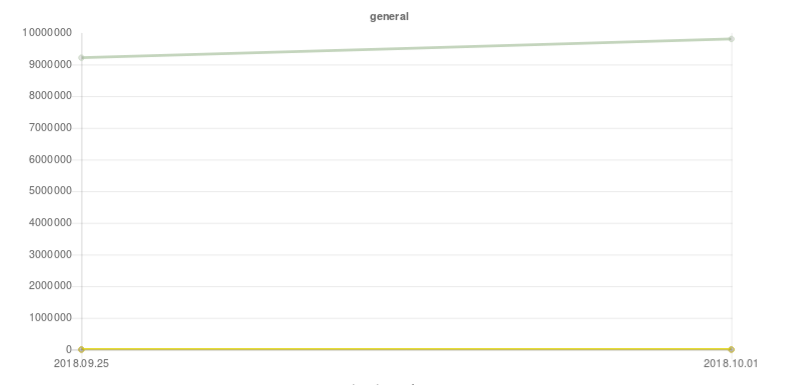
\includegraphics[width=17cm,height=8.274cm]{bilder/BilderAnalyse-img1.png}
\end{figure}
\begin{figure}
\centering
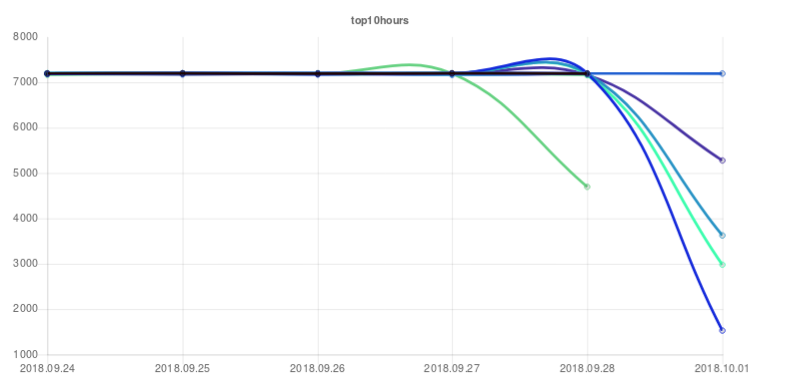
\includegraphics[width=17cm,height=8.056cm]{bilder/BilderAnalyse-img2.png}
\end{figure}
\begin{figure}
\centering
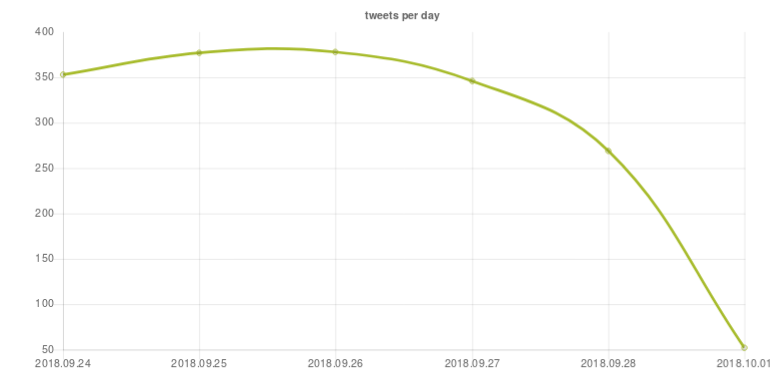
\includegraphics[width=17cm,height=8.322cm]{bilder/BilderAnalyse-img3.png}
\end{figure}

\begin{figure}
\centering
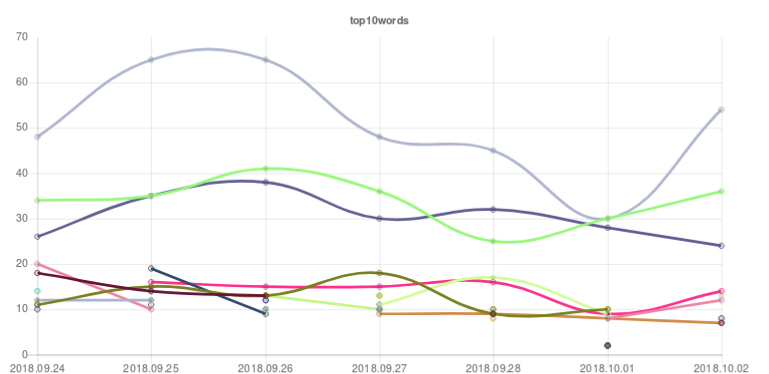
\includegraphics[width=17cm,height=8.267cm]{bilder/BilderAnalyse-img4.png}
\end{figure}
\begin{figure}
\centering
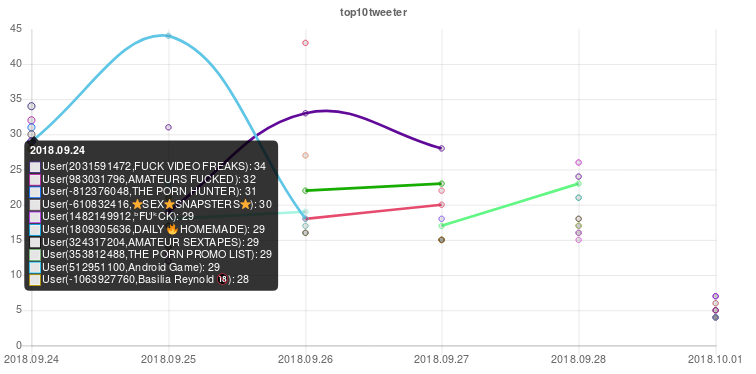
\includegraphics[width=17cm,height=8.408cm]{bilder/BilderAnalyse-img5.png}
\end{figure}
\begin{figure}
\centering
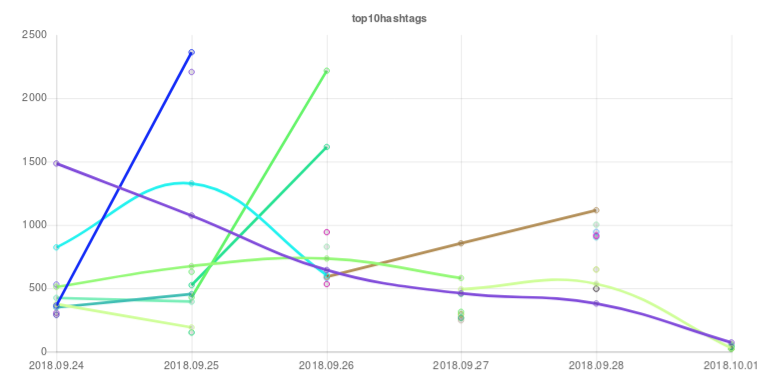
\includegraphics[width=17cm,height=8.645cm]{bilder/BilderAnalyse-img6.png}
\end{figure}


\end{document}



\section{Analytics Provisioning Service}

Für die Bereitstellung der Analysedaten ist der Micro Service \textit{Analytics Provisioning Service} zuständig. 
Dieser liest auf Anfrage Analysedaten aus Cassandra und bereitet diese für die Darstellung im Frontend auf.
In der Batchanalyse werden die Ergebnisse geordnet in einer Tabelle pro Analyse gelegt, diese werden einfach nur für die letzten 14 Tage gelesen. Ergebnisse, die weiter in der Vergangenheit liegen, werden zur Zeit nicht bereit gestellt, dies ist theoretisch aber möglich.
Da Cassandra keine Counter als sekundäre Keys unterstützt und nicht für Sortierungen von großen Datenmengen ausgelegt ist,
die Analysedaten aus dem Stream jedoch unsortiert und nicht gefiltert vorliegen, war der naive Ansatz diese mittels einer  user-defined function in Cassandra pro Anfrage zu sortieren. Dies ist aber mit steigenden Tweetzahlen sehr aufwändig und könnte z.B. durch weitere Umsetzungen mit Spark ersetzt werden.

Die Kommunikation passiert auch hier über Kafka und festgelegte Topics.
Es lassen sich beliebig viele Instanzen des Services starten, die Kommunikation skaliert automatisch über die gewählte Kommunikationsarchitektur.

Für die Umsetzung wurde die Platform Node.js mit TypeScript verwendet. 


\section{Darstellung im Frontend}

Für die Darstellung im Frontend wurde ein eigener Bereich auf der Website eingerichtet, der wiederum in die drei Teile
\textit{Live Analytics}, \textit{Batch Analytics} und Analysen von ElasticSearchs \textit{Kibana} aufgeteilt ist.
Die Analysen durch Spark werden mittels des Frameworks \textit{Graph.js} dargestellt.



\begin{figure}[htbp!]
	\centering
	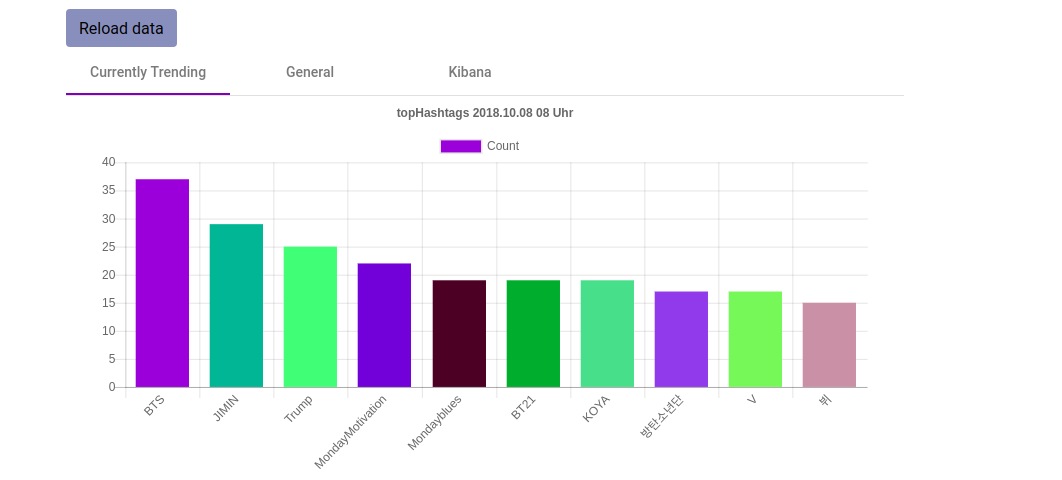
\includegraphics[width=1.1\textwidth]{pics/analytics/currentlyTrending}
	\caption{Live Analytics im Frontend}
\end{figure}
